% Requires the official AIAA/Overleaf `new-aiaa.cls` file to compile.
% Template reference:
% https://www.overleaf.com/latex/templates/preparation-of-papers-for-aiaa-technical-journals/mqqbqqvyhtwm
\documentclass[conf]{new-aiaa}

\usepackage[utf8]{inputenc}
\usepackage{textcomp}
\usepackage{graphicx}
\usepackage{amsmath}
\usepackage{amssymb}
\usepackage{booktabs}
\usepackage{longtable,tabularx}
\usepackage{subcaption}
\usepackage{siunitx}
\usepackage{url}

\setlength\LTleft{0pt}
\graphicspath{{../outputs/control_surface_sizing/rank06_n10_d5p5_p2p2_balanced_b3/}{../outputs/motor_height_trade/rank06_n10_d5p5_p2p2_balanced_b3/}}

\title{AIAA-Style Technical Note for the Blown-Wing Concept Optimizer, Rectangular-Wing High-Lift Sizing, and Motor-Height Trade Study}

\author{Nolan Nguyen\footnote{AA146 Capstone Team, Stanford University, Student Researcher.} and Codex Technical Collaborator\footnote{Automated analysis and scripting support for aerodynamic trade studies.}}
\affil{AA146 Capstone, Stanford University, Stanford, California, 94305}

\begin{document}
\maketitle

\begin{abstract}
This technical note consolidates the current implementation of the blown-wing concept optimizer, the rectangular-wing high-lift and control-surface sizing workflow, and a first motor-height trade study for a distributed-propulsion concept aircraft. Stage~1 of the optimizer performs coarse architecture screening over propeller count, diameter, pitch ratio, and prop-family surrogates while solving operating RPM internally. A downselected propulsion concept --- rank~6 in the present shortlist, corresponding to a \(10\times 5.5\times 2.2\ \mathrm{in}\) balanced propeller layout --- is then used in a higher-level rectangular-wing sizing study with single-slotted flaps and cruise ailerons. The current low-speed configuration assumes maximum slotted-flap deflection, propellers located ahead of the flap region, and a lowered prop centerline to reflect favorable flap interaction observed qualitatively in the literature. Finally, a constrained trade study sweeps motor vertical offset to quantify how propeller drop affects equivalent whole-wing high-lift capability. The note is intentionally implementation-matched: equations and figures correspond to the current repository outputs rather than to a generic conceptual model.
\end{abstract}

\section*{Nomenclature}
\begin{longtable*}{@{}ll@{}}
\(A_{\mathrm{disk}}\) & total propeller disk area \\
\(AR\) & wing aspect ratio \\
\(C_D\) & drag coefficient \\
\(C_{D0}\) & zero-lift drag coefficient \\
\(C_L\) & lift coefficient referenced to the full wing and freestream dynamic pressure \\
\(C_l\) & local section lift coefficient \\
\(C_\mu\) & wing-reference momentum coefficient \\
\(C_P\) & propeller power coefficient \\
\(C_T\) & propeller thrust coefficient \\
\(D\) & propeller diameter or drag force, by context \\
\(e\) & Oswald efficiency factor \\
\(\eta_b\) & blown span fraction \\
\(n\) & propeller rotational speed in revolutions per second \\
\(P/D\) & propeller pitch ratio \\
\(q\) & dynamic pressure \\
\(Re\) & Reynolds number \\
\(S\) & wing reference area \\
\(S_b\) & blown wing area \\
\(S_u\) & unblown wing area \\
\(T\) & thrust \\
\(V_\infty\) & freestream velocity \\
\(V_{\mathrm{eff}}\) & slipstream-enhanced effective velocity over the blown region \\
\(v_i\) & actuator-disk induced velocity \\
\end{longtable*}

\section{Introduction}

The present design problem is to identify a propulsion architecture and high-lift configuration that can support very low-speed flight on a fixed-span wing while maintaining acceptable cruise behavior. The repository now contains three connected levels of modeling:
\begin{enumerate}
\item a Stage~1 coarse architecture screen,
\item a rectangular-wing slotted-flap and aileron sizing workflow for a chosen propulsion concept, and
\item a first-order motor-height trade study based on that same concept.
\end{enumerate}

The immediate motivation for the present note is twofold. First, the current codebase had reached a point where equations, assumptions, and outputs needed to be synchronized in one manuscript. Second, raw section-polars alone were proving misleading when interpreting the benefit of blowing: the strongest low-speed benefit is not simply a higher section \(C_l\), but rather the combination of modest local \(C_l\) improvement with a large increase in local dynamic pressure.

\section{Stage~1 Architecture Screen}

\subsection{Design variables and fixed assumptions}

Stage~1 evaluates the discrete design space
\begin{equation}
\mathbf{x} =
\left\{
N_p,\;
D,\;
\frac{P}{D},\;
f_{\mathrm{prop}}
\right\},
\end{equation}
with
\begin{align}
N_p &\in \{4,6,8,10,12,14,16\}, \\
D &\in \{4.0,4.5,5.0,5.5,6.0,6.5,7.0,7.5,8.0,9.0,10.0\}\ \mathrm{in}, \\
\frac{P}{D} &\in \{0.40,0.50,0.60,0.70,0.80,0.90\}, \\
f_{\mathrm{prop}} &\in \{\texttt{high\_thrust},\texttt{balanced},\texttt{cruise}\}.
\end{align}

The global mission assumptions used in the present implementation are:
\begin{itemize}
\item gross mass \(m_{\mathrm{gross}} = \SI{5.0}{kg}\),
\item span \(b = \SI{2.0}{m}\),
\item baseline chord \(c = \SI{0.35}{m}\),
\item low-speed design condition \(V_{\infty,\mathrm{low}} = \SI{4.0}{m/s}\),
\item cruise condition \(V_{\infty,\mathrm{cruise}} = \SI{10.0}{m/s}\),
\item battery voltage \(V_{\mathrm{batt}} = \SI{14.8}{V}\),
\item battery specific energy \(\epsilon_{\mathrm{batt}} = \SI{180}{Wh/kg}\), and
\item wing-system working ceiling \(C_{L,\mathrm{ceil}} = 2.0\).
\end{itemize}

\subsection{Propeller surrogate and operating-point solve}

The propeller surrogate remains a coarse architecture model. For a given propeller family, pitch ratio, and advance ratio \(J\),
\begin{equation}
J = \frac{V}{nD},
\qquad
n = \frac{\mathrm{RPM}}{60},
\end{equation}
the code constructs effective \(C_T\) and \(C_P\) values and then computes
\begin{align}
T_{\mathrm{per}} &= C_T \rho n^2 D^4, \\
P_{\mathrm{shaft,per}} &= C_P \rho n^3 D^5.
\end{align}
Total thrust and shaft power are
\begin{align}
T_{\mathrm{tot}} &= N_p T_{\mathrm{per}}, \\
P_{\mathrm{shaft,tot}} &= N_p P_{\mathrm{shaft,per}}.
\end{align}

Unlike the earliest grid-based version, RPM is no longer treated as an outer design variable. Stage~1 solves the low-speed and cruise RPMs internally with bisection so that each architecture is compared at its minimum feasible operating point.

\subsection{Blown-wing low-speed model}

The wing is partitioned into blown and unblown areas:
\begin{align}
S_b &= \eta_b S, \\
S_u &= (1-\eta_b)S.
\end{align}
The total disk area is
\begin{equation}
A_{\mathrm{disk}} = N_p \pi \left(\frac{D}{2}\right)^2.
\end{equation}
Stage~1 uses an actuator-disk relation to estimate the effective blown velocity:
\begin{align}
v_i &= \sqrt{\frac{T_{\mathrm{tot}}}{2 \rho A_{\mathrm{disk}}}}, \\
V_{\mathrm{eff}} &= V_\infty + 2v_i.
\end{align}
For the selected rank-6 concept discussed later,
\begin{equation}
V_{\mathrm{eff}} = \SI{14.622}{m/s}, \qquad
v_i = \SI{5.311}{m/s},
\end{equation}
at the low-speed condition \(V_\infty = \SI{4.0}{m/s}\).

Stage~1 also defines a wing-reference momentum coefficient,
\begin{equation}
C_\mu = \frac{T_{\mathrm{tot}}}{q_\infty S},
\end{equation}
and uses it in a clipped blown-section lift-augmentation model. However, because the current wing-system ceiling is held to \(C_{L,\mathrm{ceil}} = 2.0\), the dominant benefit of blowing at low speed is not a large rise in local section \(C_l\), but the increase in local dynamic pressure on the blown region.

\section{Rectangular-Wing High-Lift and Control-Surface Sizing}

\subsection{Configuration and assumptions}

The follow-on sizing study freezes the planform to a rectangular wing with
\begin{equation}
b = \SI{2.0}{m},
\qquad
c = \SI{0.35}{m},
\qquad
S = \SI{0.70}{m^2}.
\end{equation}
The selected propulsion concept is the current rank-6 architecture:
\begin{equation}
10 \times 5.5 \times 2.2\ \mathrm{in},
\end{equation}
with a balanced propeller family and three-blade metadata.

At low speed, the slotted flap is assumed to be fully deployed at its maximum deflection. In the current implementation, that means
\begin{equation}
\delta_f = \SI{40}{deg}.
\end{equation}
The propellers that lie ahead of the flap span are also assumed to sit slightly below the wing chord line. The present baseline drop is
\begin{equation}
\Delta z_p = 0.12 D = \SI{0.0168}{m},
\end{equation}
which is represented in the code through a heuristic prop-drop bonus applied only to the blown flap section.

\subsection{Section-polar construction}

The flap-sizing script first evaluates clean and flapped section polars with NeuralFoil, then applies a mild slot-gain correction:
\begin{equation}
C_{l,\mathrm{flapped,adj}}
=
C_{l,\mathrm{clean}}

+ f_{\mathrm{slot}}
\left(
C_{l,\mathrm{raw\ flap}} - C_{l,\mathrm{clean}}
\right).
\end{equation}
The slot-gain factor is a heuristic function of flap chord ratio, deflection, and prop-drop bonus. It is deliberately modest in the current model. As a result, the raw section lift curves do not show an enormous upward translation of \(C_l(\alpha)\). This is intentional: the code presently attributes the main low-speed benefit of blowing to local dynamic-pressure rise rather than to extreme section \(C_l\) augmentation.

\subsection{Why section curves alone are misleading}

For the selected concept,
\begin{equation}
\frac{q_b}{q_\infty}
=
\left(\frac{V_{\mathrm{eff}}}{V_\infty}\right)^2
=
\left(\frac{14.622}{4.0}\right)^2
\approx 13.36.
\end{equation}
Thus a comparatively small increase in local section \(C_l\) on the blown flap region can still produce a large increase in whole-wing equivalent \(C_L\), simply because the local blown region sees more than thirteen times the freestream dynamic pressure.

\section{Results for the Selected Rank-6 Concept}

\subsection{Recommended flap and aileron geometry}

The current rectangular-wing sizing recommendation is:
\begin{itemize}
\item flap span fraction \(= 0.60\) of semispan,
\item flap chord fraction \(= 0.22\),
\item flap deflection \(= \SI{40}{deg}\),
\item aileron span fraction \(= 0.28\) of semispan,
\item aileron chord fraction \(= 0.28\).
\end{itemize}

The corresponding low-speed and control metrics are:
\begin{itemize}
\item equivalent reference \(C_{L,\max} = 16.657\),
\item equivalent stall speed \(V_s = \SI{2.620}{m/s}\),
\item low-speed lift margin at \(\SI{4}{m/s}\): \(133.0\%\),
\item estimated roll rate at \(\delta_a = \SI{14}{deg}\): \(\SI{30.9}{deg/s}\),
\item estimated roll rate at \(\delta_a = \SI{20}{deg}\): \(\SI{44.1}{deg/s}\).
\end{itemize}

\begin{figure}[t]
    \centering
    
\includegraphics[width=0.92\linewidth]{layout.png}
    \caption{Rectangular-wing layout used in the control-surface sizing workflow. The inboard single-slotted flaps are shown in orange, the outboard ailerons in blue, and the propeller disks as dashed circles. The right-hand panel illustrates the baseline prop drop relative to the flap chord line.}
    \label{fig:layout}
\end{figure}

\begin{figure}[t]
    \centering
    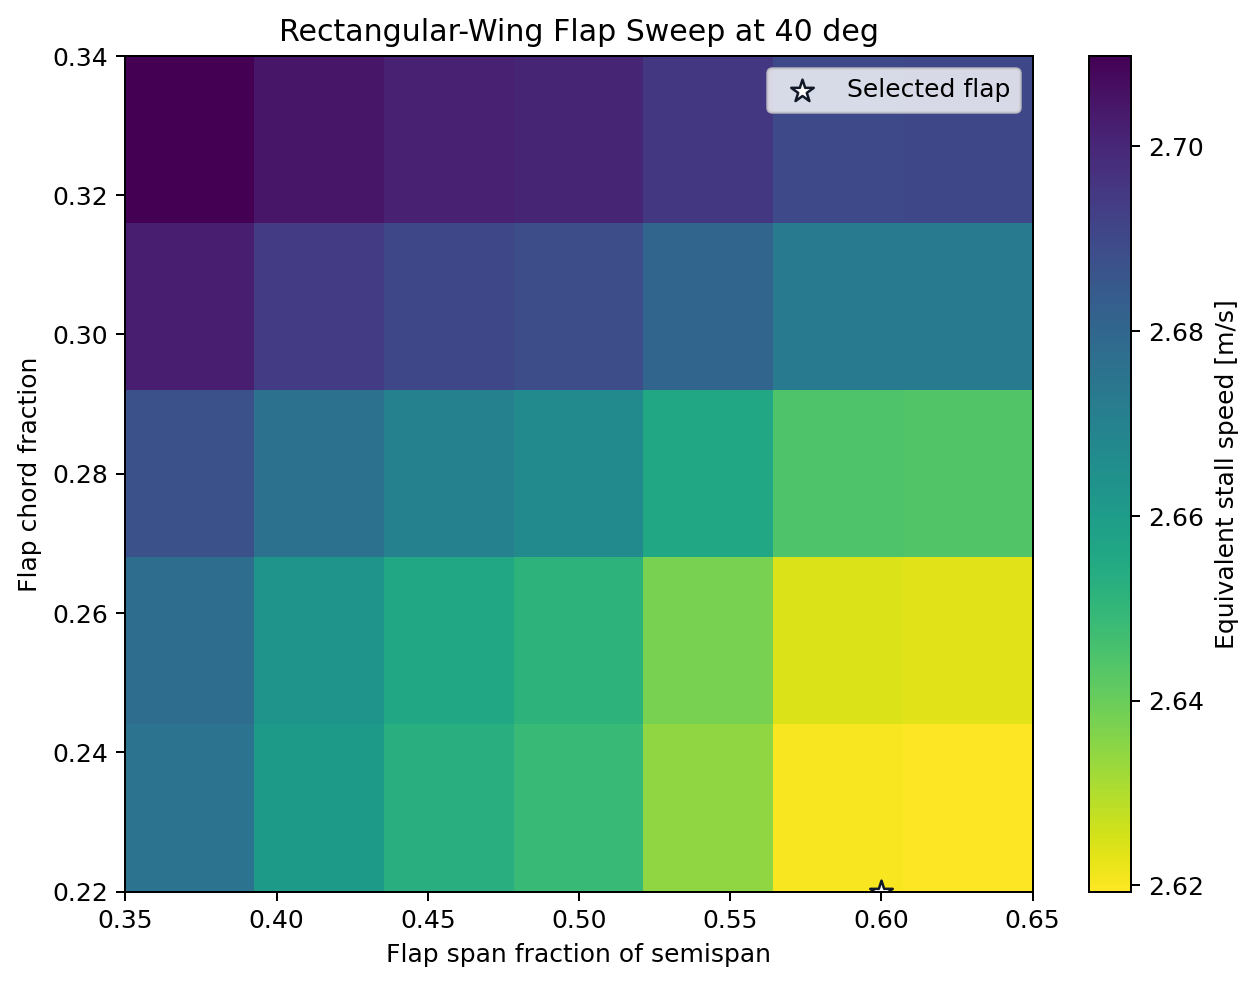
\includegraphics[width=0.92\linewidth]{flap_heatmap.png}
    \caption{Flap-design heatmap at the maximum low-speed flap deflection. The selected configuration occurs at \(60\%\) semispan and \(c_f/c=0.22\), where the equivalent stall speed is minimized under the current constraints.}
    \label{fig:flap_heatmap}
\end{figure}

\begin{figure}[t]
    \centering
    
\includegraphics[width=0.92\linewidth]{flap_section_polars.png}
    \caption{Section polars used in the flap-sizing study. These curves should not be over-interpreted as the total aircraft benefit of blowing. In the current model, the strongest low-speed gain enters through the increased blown-region dynamic pressure rather than through a dramatic increase in section \(C_l\) by itself.}
    \label{fig:section_polars}
\end{figure}

\begin{figure}[t]
    \centering
    
\includegraphics[width=0.92\linewidth]{total_cl_curve.png}
    \caption{Whole-wing equivalent \(C_L\) curves referenced to freestream dynamic pressure. This is the more appropriate interpretation plot for the present blown-wing model. The ``all high-lift active'' curve includes flap deflection, blowing, and the prop-drop bonus simultaneously.}
    \label{fig:total_cl}
\end{figure}

\begin{figure}[t]
    \centering
    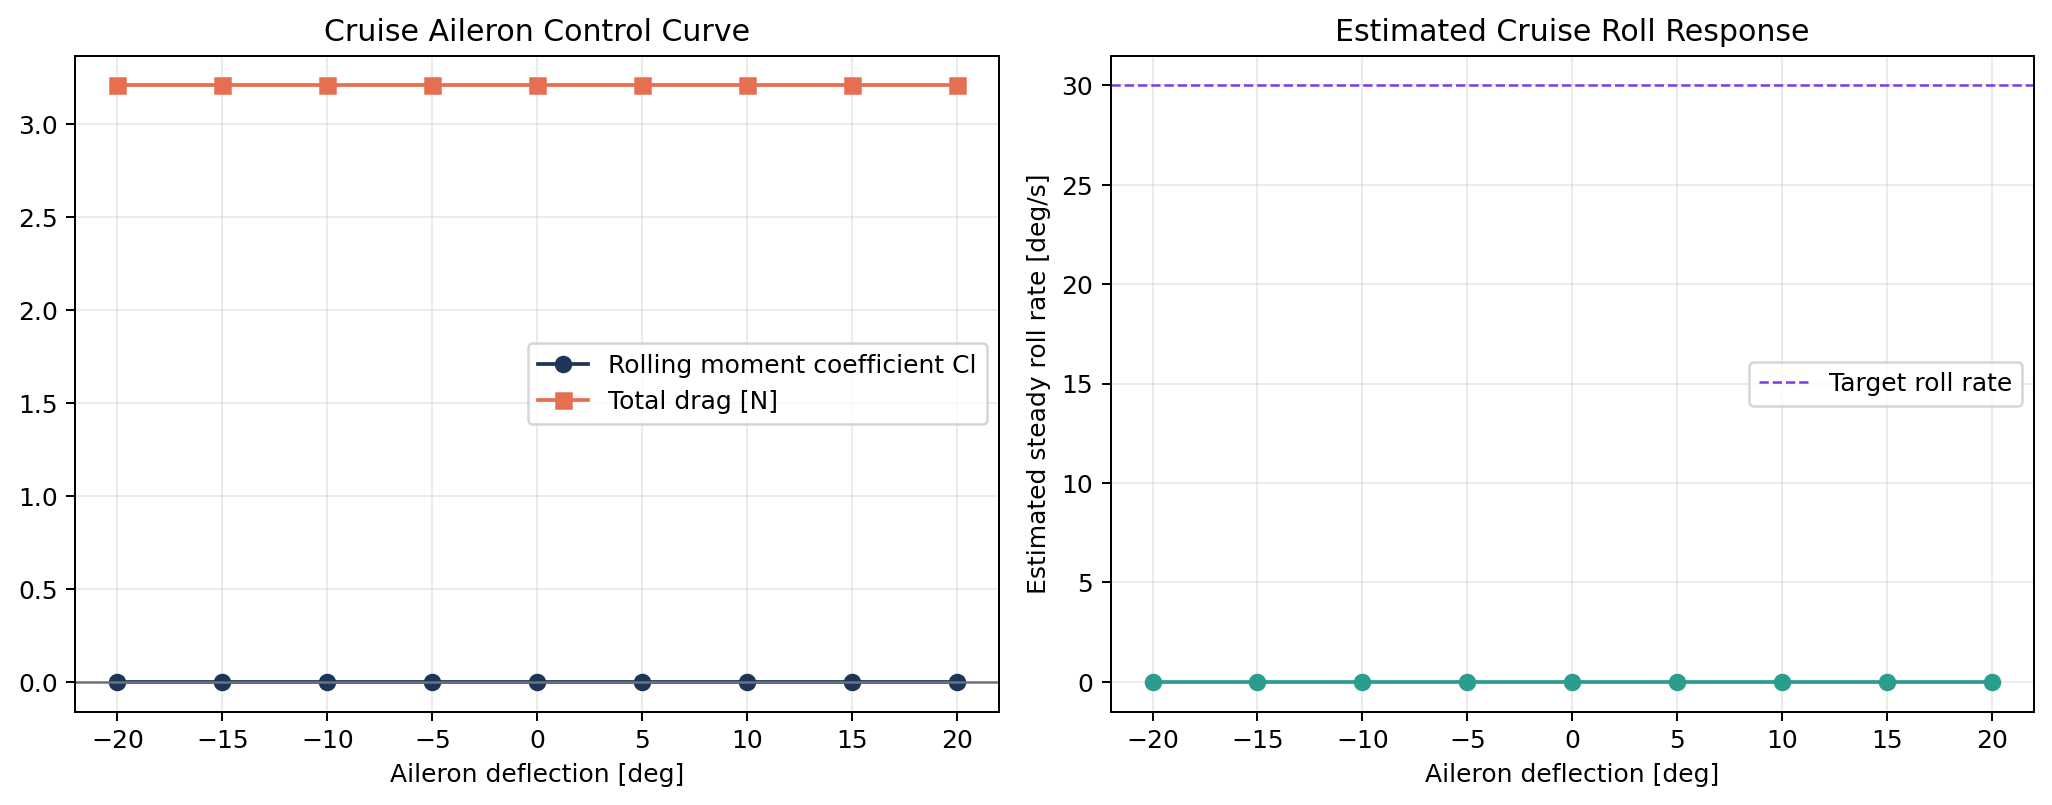
\includegraphics[width=0.92\linewidth]{aileron_curves.png}
    \caption{Cruise aileron response for the selected rectangular-wing geometry. The rolling-moment response is modest but monotonic, and the derived roll-rate estimate is sufficient to meet the current internal target of \(\SI{30}{deg/s}\).}
    \label{fig:aileron_curves}
\end{figure}

\subsection{Interpretation}

Two observations are important. First, the current model predicts that the aircraft can satisfy the \(\SI{4}{m/s}\) lift requirement with substantial margin once the blown-flap system is active. Second, the raw section polar does not visually capture the main system-level benefit of blowing. Figure~\ref{fig:total_cl}, not Fig.~\ref{fig:section_polars}, is therefore the appropriate diagnostic for judging whether the high-lift system is helping the entire wing.

\section{Motor-Height Trade Study}

\subsection{Trade formulation}

To isolate the effect of motor vertical position, the selected rank-6 propulsion architecture and the selected flap/aileron geometry are held fixed while the propeller vertical drop is swept. The present study uses the following nondimensional motor-drop values:
\begin{equation}
\frac{\Delta z_p}{D} \in \{0.00, 0.04, 0.08, 0.12, 0.16, 0.20, 0.24\}.
\end{equation}

The current script translates motor height into performance through a bounded prop-drop bonus multiplier,
\begin{equation}
f_{\mathrm{drop}}
=
1 + \Delta_{\mathrm{drop}}
\exp\left[
-\left(
\frac{\Delta z_p/D - (\Delta z_p/D)_{\mathrm{peak}}}{w_{\mathrm{drop}}}
\right)^2
\right],
\end{equation}
with
\begin{equation}
\Delta_{\mathrm{drop}} = 0.03,\quad
\left(\frac{\Delta z_p}{D}\right)_{\mathrm{peak}} = 0.12,\quad
w_{\mathrm{drop}} = 0.08.
\end{equation}
This is a concept-level surrogate: it is meant to represent the qualitative notion that some downward prop offset can improve flap interaction, but that the benefit should diminish if the propeller is either too high or too low.

\subsection{Trade results}

The resulting summary shows a shallow optimum near the baseline drop. In the present model:
\begin{itemize}
\item the best equivalent stall speed occurs at a motor drop of approximately \SI{17}{mm},
\item the equivalent reference \(C_{L,\max}\) also peaks near that same drop,
\item the roll-rate estimate is essentially unchanged across the sweep because the aileron geometry is held fixed and the trade acts primarily through the blown flap region.
\end{itemize}

\begin{figure}[t]
    \centering
    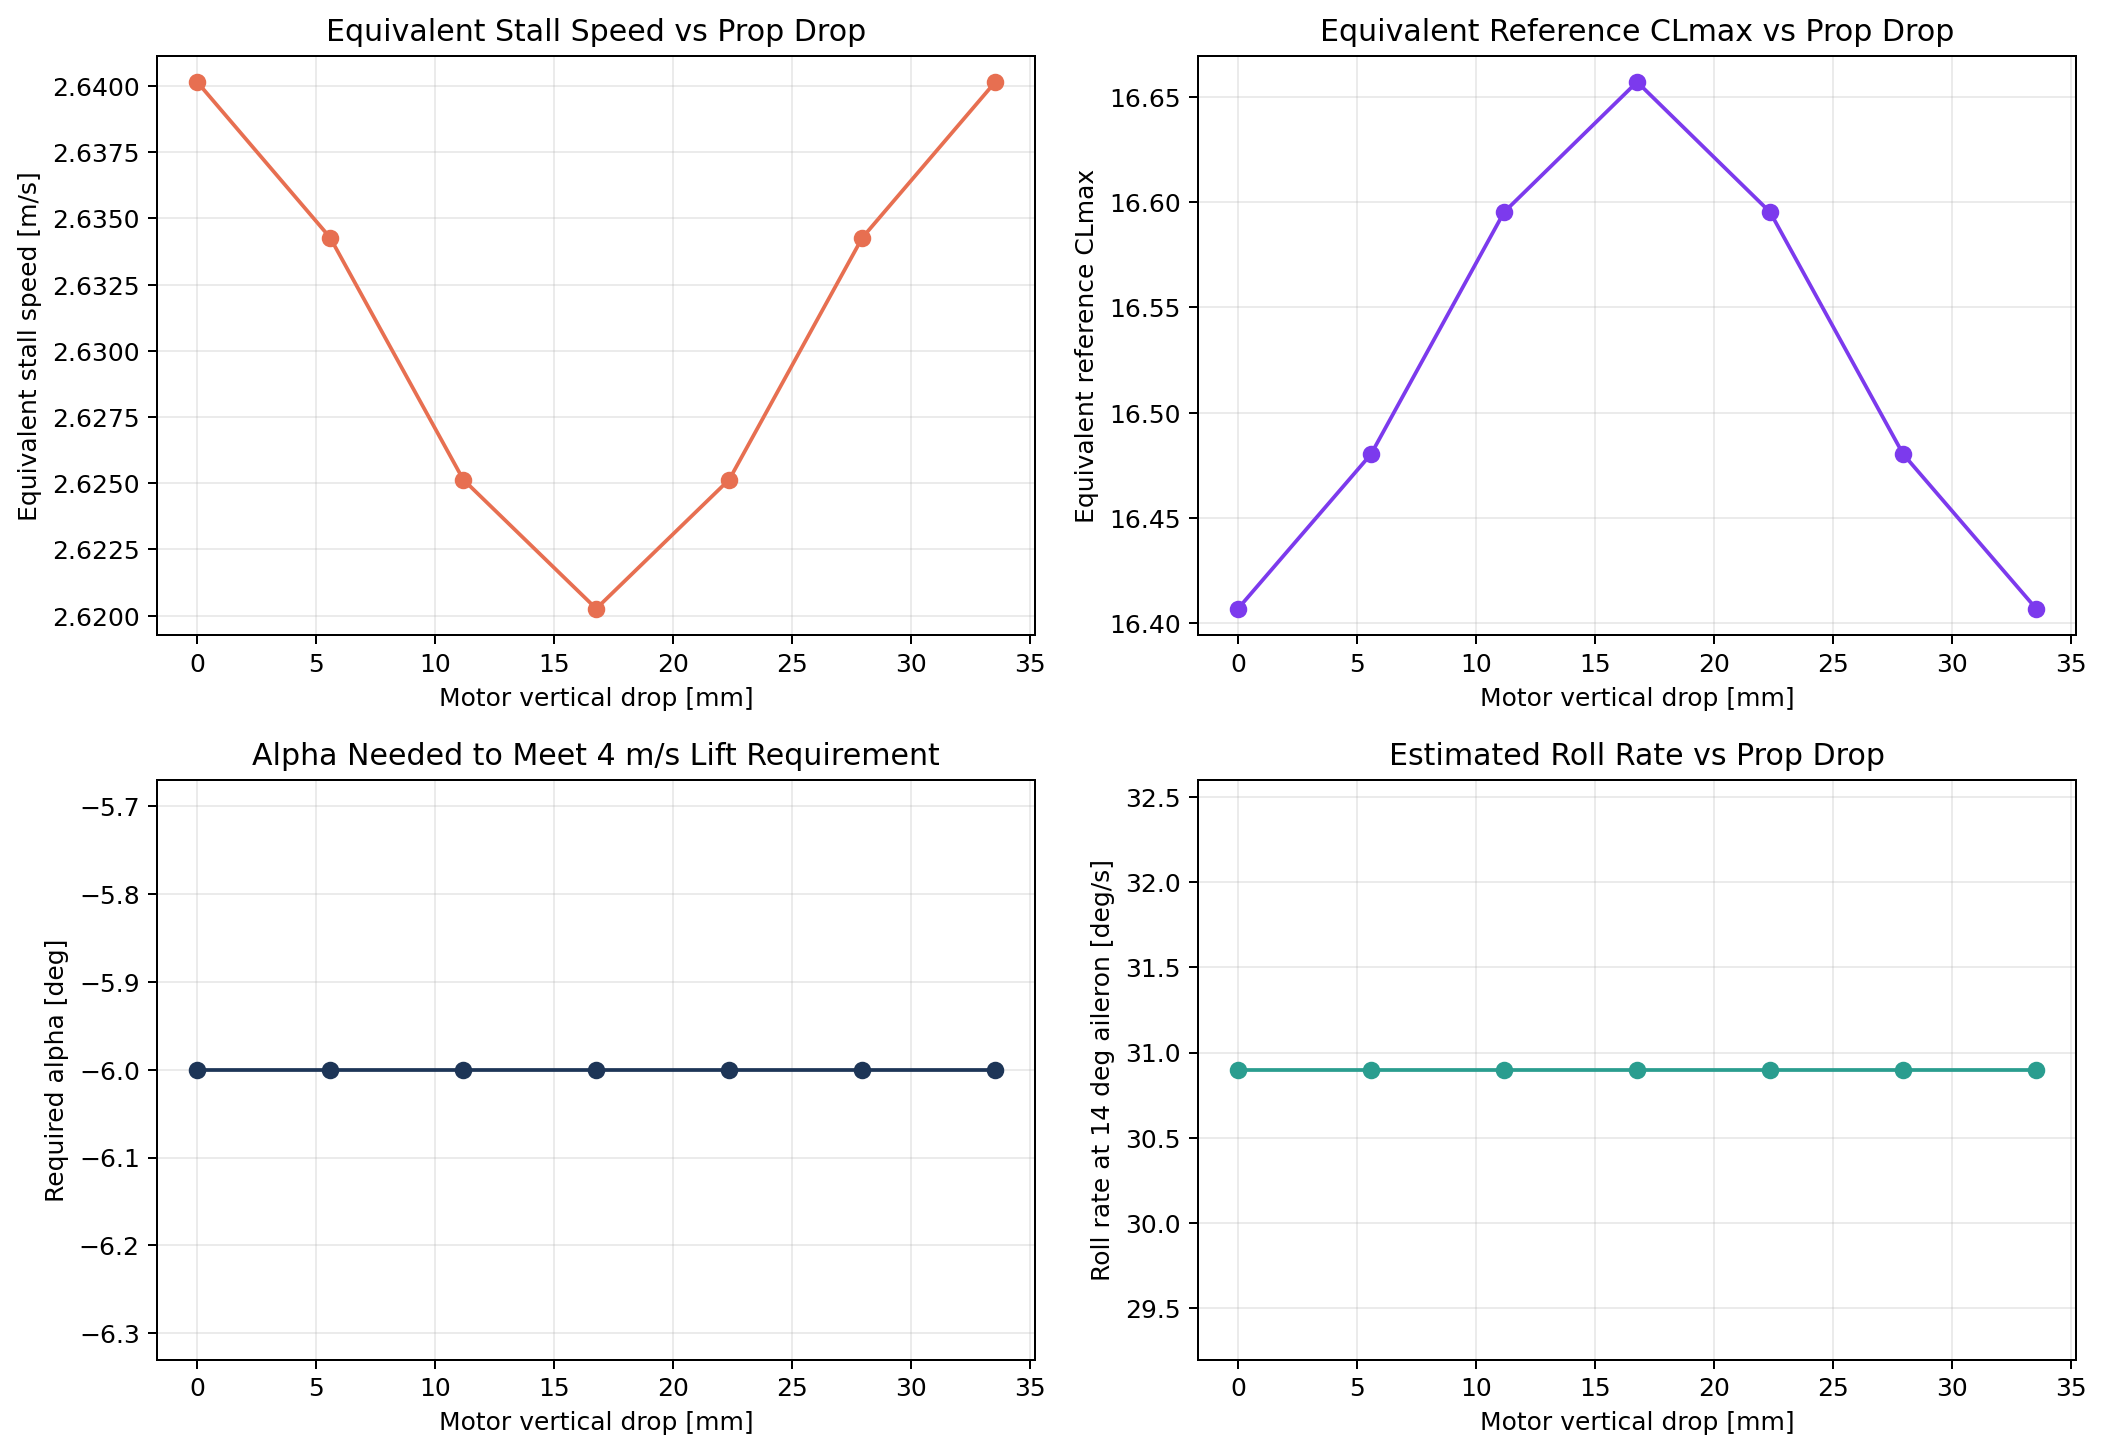
\includegraphics[width=0.92\linewidth]{motor_height_trade_metrics.png}
    \caption{Motor-height trade metrics for the selected rank-6 concept. Within the present surrogate, a moderate drop improves equivalent low-speed performance slightly, while the overall sensitivity remains fairly shallow.}
    \label{fig:trade_metrics}
\end{figure}

\begin{figure}[t]
    \centering
    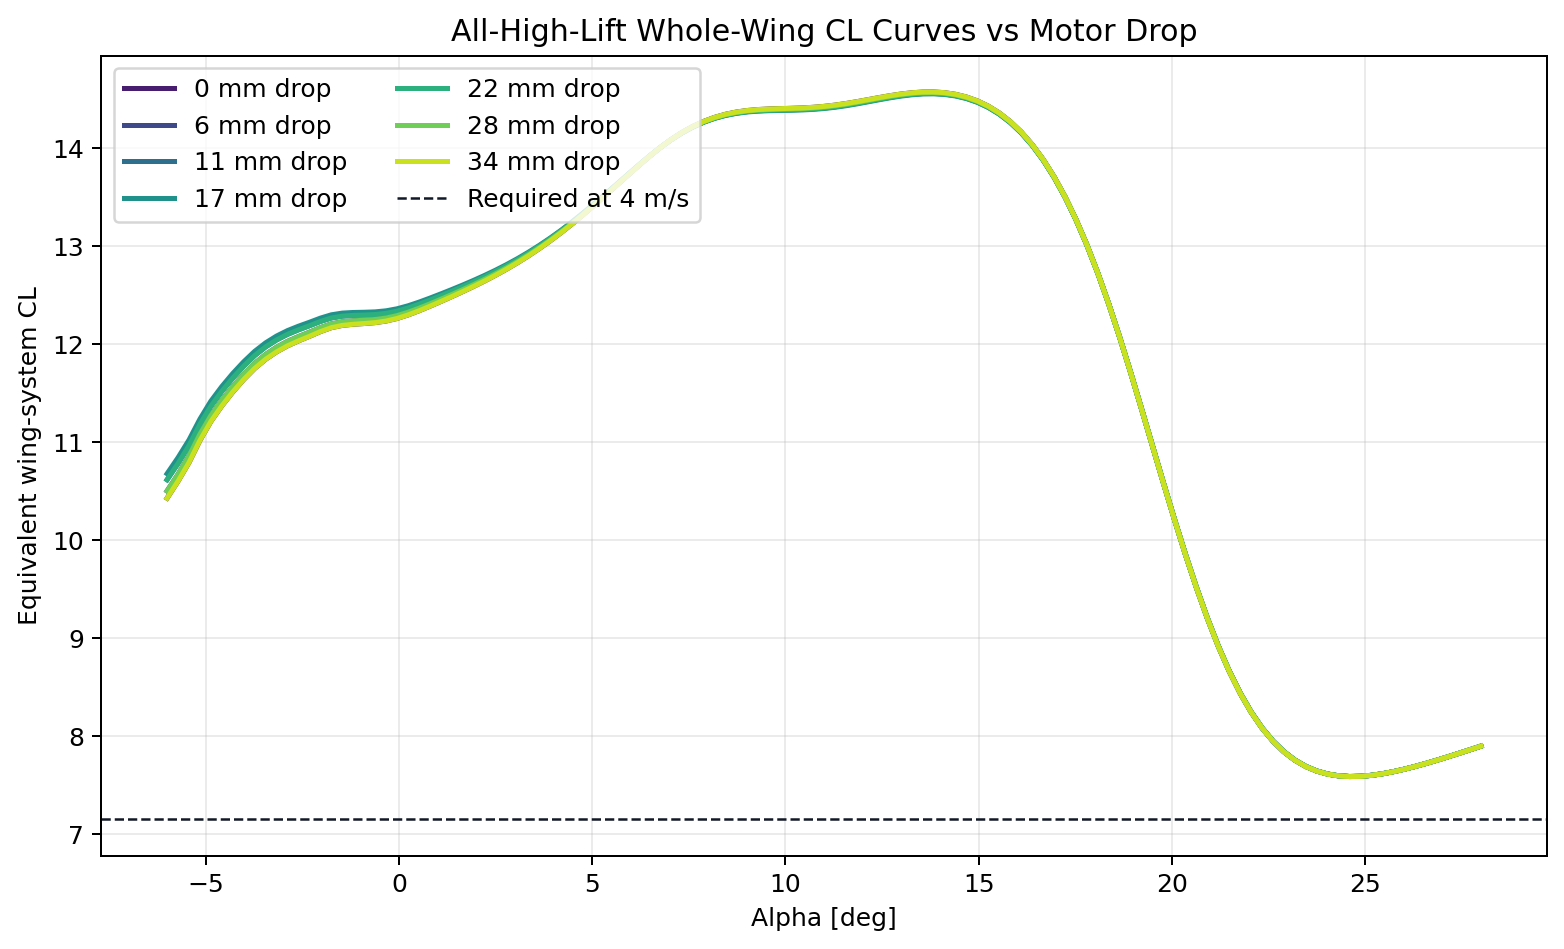
\includegraphics[width=0.92\linewidth]{motor_height_trade_cl_overlay.png}
    \caption{Overlay of whole-wing all-high-lift \(C_L\) curves for several motor-drop values. The effect of vertical offset is modest in the current implementation because it enters only through the bounded prop-drop bonus applied to the blown flap section.}
    \label{fig:trade_overlay}
\end{figure}

\begin{figure}[t]
    \centering
    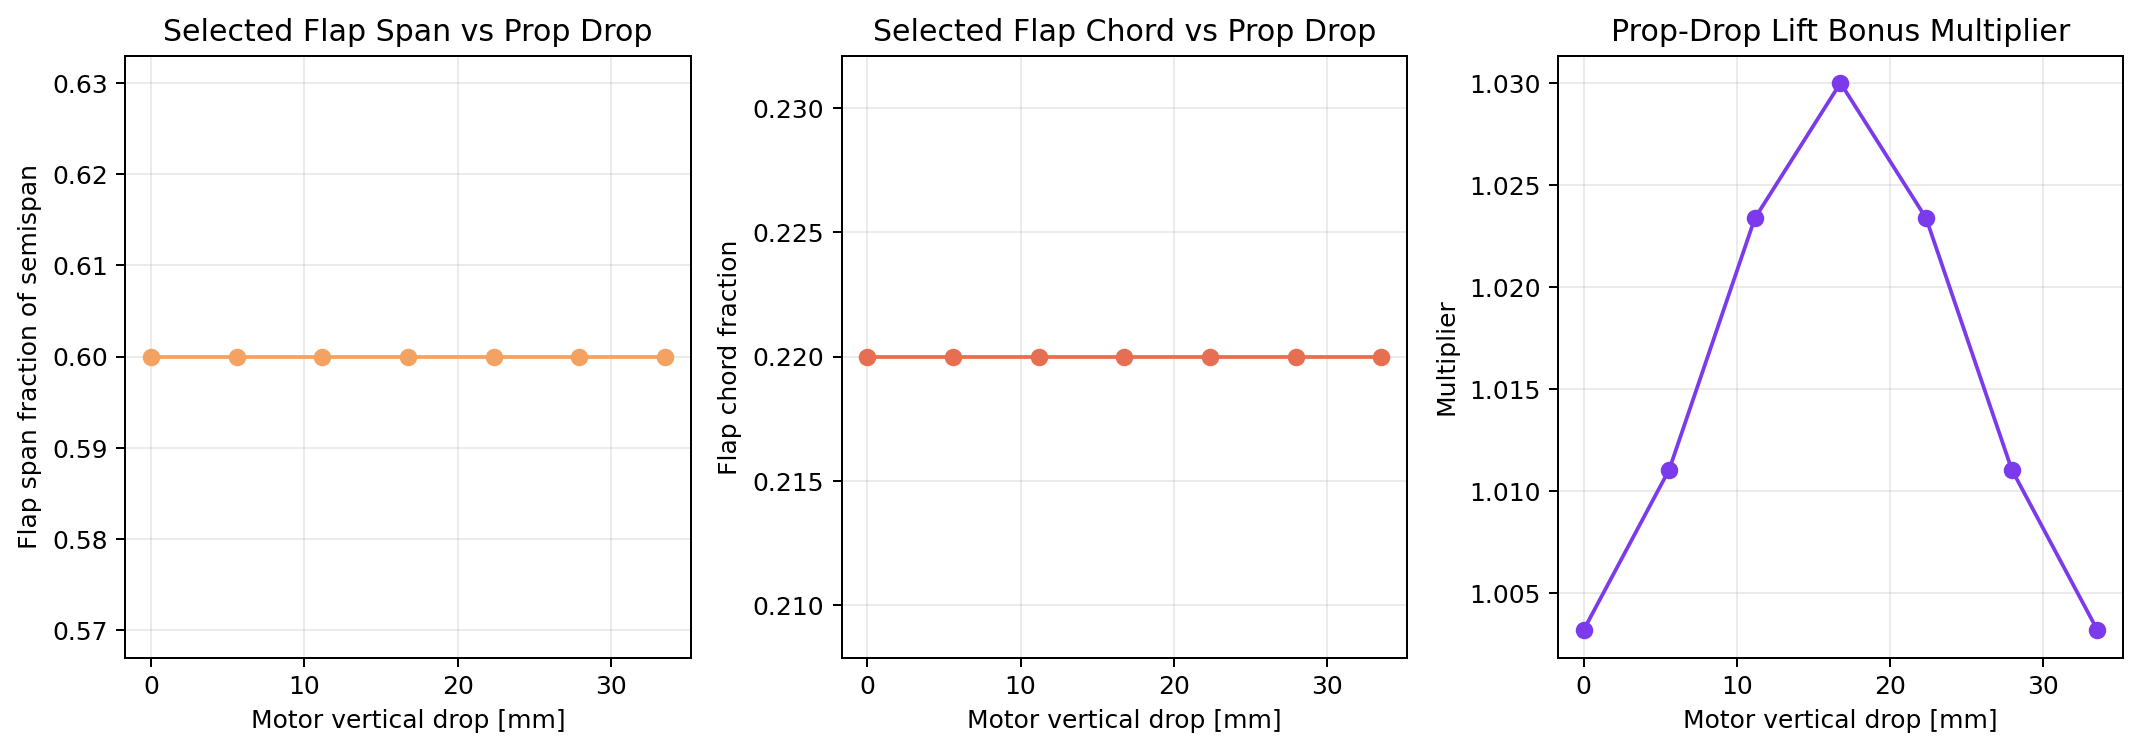
\includegraphics[width=0.92\linewidth]{motor_height_trade_geometry.png}
    \caption{Selected geometry and bonus terms across the motor-height sweep. The flap geometry is held fixed for the present one-variable trade, while the drop bonus peaks near the baseline \(\Delta z_p/D = 0.12\).}
    \label{fig:trade_geometry}
\end{figure}

\subsection{Interpretation and limitations}

The current trade should be interpreted as a first-order sensitivity study, not as a final geometric optimum. It provides three useful insights:
\begin{enumerate}
\item The code now has a structured way to compare motor height as a design variable.
\item The baseline prop drop remains reasonable under the present assumptions.
\item The trade is currently limited by the simplicity of the drop surrogate.
\end{enumerate}

The largest remaining modeling gap is that motor height does not yet alter the actual slipstream footprint or incidence over the flap geometry in a resolved flowfield sense. A higher-fidelity follow-on study should therefore replace the present bounded bonus with a CFD-calibrated or experiment-calibrated relationship.

\section{Conclusions}

The repository now contains a coherent path from coarse propulsion downselection to rectangular-wing high-lift sizing and, finally, to a first motor-height sensitivity study. The main technical conclusions are:
\begin{itemize}
\item The Stage~1 blown-wing architecture screen is mathematically well defined and suitable for concept downselection.
\item For the selected rank-6 propulsion concept, the current rectangular-wing study supports a \(60\%\)-semispan single-slotted flap at \(c_f/c=0.22\) and \(\delta_f=\SI{40}{deg}\), together with a \(28\%\)-semispan aileron at \(c_a/c=0.28\).
\item The most informative low-speed diagnostic is the whole-wing equivalent \(C_L\) curve, not the raw section \(C_l(\alpha)\) plot.
\item The present motor-height trade indicates a mild performance preference for a moderate downward prop offset near \(\Delta z_p/D \approx 0.12\), though the sensitivity remains small under the current surrogate.
\end{itemize}

\section*{References}
\begin{thebibliography}{99}
\bibitem{AIAATemplate}
AIAA and Overleaf,
``Preparation of Papers for AIAA Technical Journals,''
Overleaf official template,
\url{https://www.overleaf.com/latex/templates/preparation-of-papers-for-aiaa-technical-journals/mqqbqqvyhtwm},
accessed Apr. 22, 2026.

\bibitem{AIAALaTeXTips}
American Institute of Aeronautics and Astronautics,
``Tips for \LaTeX{} Authors,''
\url{https://aiaa.org/publications/journals/journal-author/tips-for-latex-authors/},
accessed Apr. 22, 2026.

\bibitem{Long2021}
Long, T., Drela, M., Hansman, R. J., and Courtin, C.,
``An Experimental Investigation of a Blown-Flap Wing,''
\emph{AIAA AVIATION 2021 FORUM},
AIAA Paper 2021-2871,
2021.

\bibitem{Plijter2025}
Plijter, J. C., Duivenvoorden, R. R., and Sinnige, T.,
``Aerodynamic Interaction Effects Between a Propeller Slipstream and Single Slotted Flap,''
\emph{AIAA SCITECH 2025 Forum},
AIAA Paper 2025-0667,
2025.

\bibitem{Maki1959}
Maki, R. L.,
``Low-Speed Wind-Tunnel Investigation of Blowing Boundary-Layer Control on Leading- and Trailing-Edge Flaps of a Large-Scale, Low-Aspect-Ratio, 45 Swept-Wing Airplane Configuration,''
NASA Memorandum 1-23-59A,
1959.
\end{thebibliography}

\end{document}
